% Created by tikzDevice version 0.12.6 on 2026-05-29 11:03:03
% !TEX encoding = UTF-8 Unicode
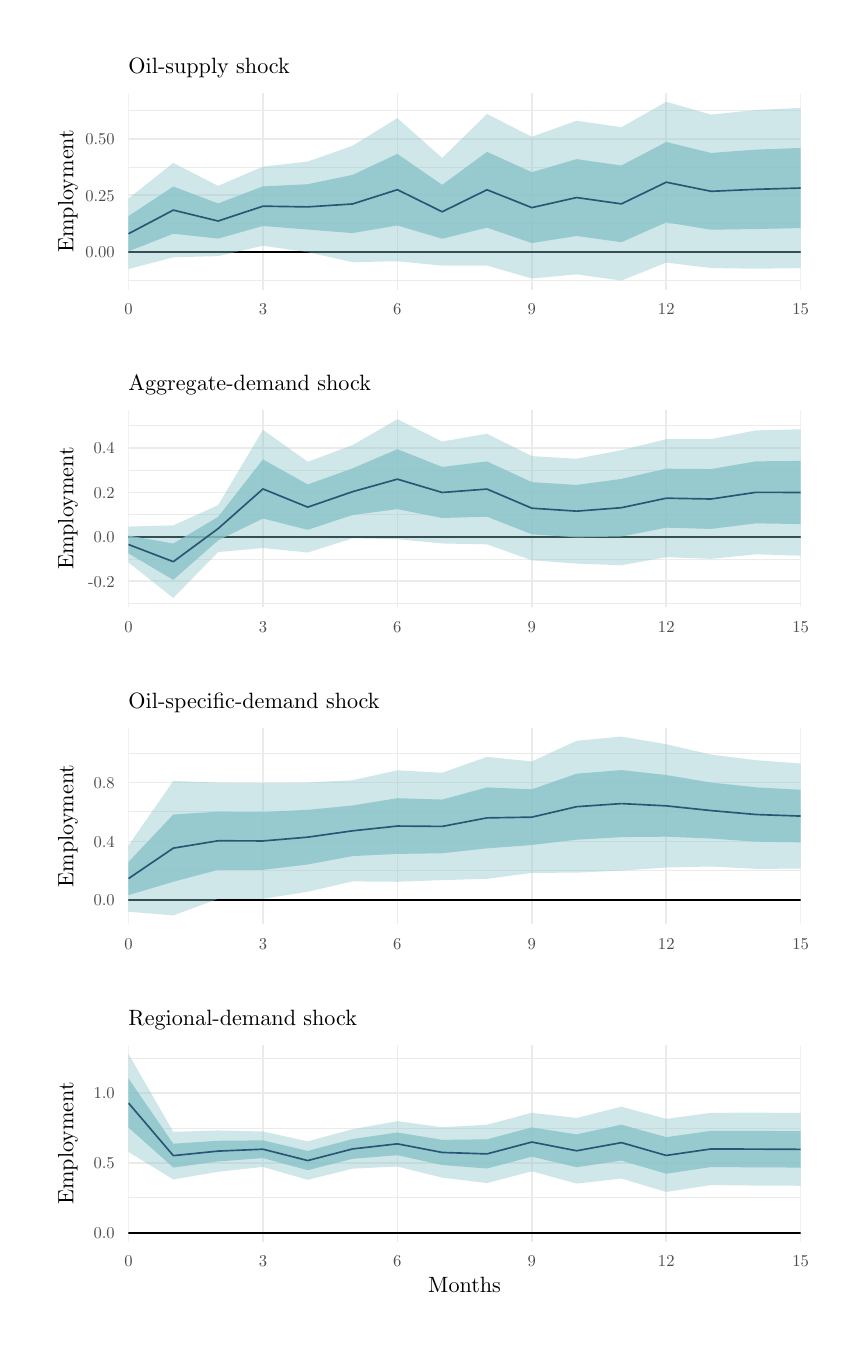
\begin{tikzpicture}[x=1pt,y=1pt]
\definecolor{fillColor}{RGB}{255,255,255}
\path[use as bounding box,fill=fillColor,fill opacity=0.00] (0,0) rectangle (290.32,469.75);
\begin{scope}
\path[clip] (  0.00,  0.00) rectangle (290.32,469.75);
\definecolor{drawColor}{RGB}{255,255,255}
\definecolor{fillColor}{RGB}{255,255,255}

\path[draw=drawColor,line width= 0.6pt,line join=round,line cap=round,fill=fillColor] (  0.00,  0.00) rectangle (290.32,469.76);
\end{scope}
\begin{scope}
\path[clip] (  5.50,349.57) rectangle (284.82,464.26);
\definecolor{fillColor}{RGB}{255,255,255}

\path[fill=fillColor] (  5.50,349.57) rectangle (284.82,464.26);
\end{scope}
\begin{scope}
\path[clip] (  5.50,234.88) rectangle (284.82,349.57);
\definecolor{fillColor}{RGB}{255,255,255}

\path[fill=fillColor] (  5.50,234.88) rectangle (284.82,349.57);
\end{scope}
\begin{scope}
\path[clip] (  5.50,120.19) rectangle (284.82,234.88);
\definecolor{fillColor}{RGB}{255,255,255}

\path[fill=fillColor] (  5.50,120.19) rectangle (284.82,234.88);
\end{scope}
\begin{scope}
\path[clip] (  5.50,  5.50) rectangle (284.82,120.19);
\definecolor{fillColor}{RGB}{255,255,255}

\path[fill=fillColor] (  5.50,  5.50) rectangle (284.82,120.19);
\end{scope}
\begin{scope}
\path[clip] ( 36.43,375.13) rectangle (279.32,446.19);
\definecolor{drawColor}{gray}{0.92}

\path[draw=drawColor,line width= 0.3pt,line join=round] ( 36.43,378.57) --
	(279.32,378.57);

\path[draw=drawColor,line width= 0.3pt,line join=round] ( 36.43,398.97) --
	(279.32,398.97);

\path[draw=drawColor,line width= 0.3pt,line join=round] ( 36.43,419.37) --
	(279.32,419.37);

\path[draw=drawColor,line width= 0.3pt,line join=round] ( 36.43,439.77) --
	(279.32,439.77);

\path[draw=drawColor,line width= 0.6pt,line join=round] ( 36.43,388.77) --
	(279.32,388.77);

\path[draw=drawColor,line width= 0.6pt,line join=round] ( 36.43,409.17) --
	(279.32,409.17);

\path[draw=drawColor,line width= 0.6pt,line join=round] ( 36.43,429.57) --
	(279.32,429.57);

\path[draw=drawColor,line width= 0.6pt,line join=round] ( 36.43,375.13) --
	( 36.43,446.19);

\path[draw=drawColor,line width= 0.6pt,line join=round] ( 85.01,375.13) --
	( 85.01,446.19);

\path[draw=drawColor,line width= 0.6pt,line join=round] (133.59,375.13) --
	(133.59,446.19);

\path[draw=drawColor,line width= 0.6pt,line join=round] (182.17,375.13) --
	(182.17,446.19);

\path[draw=drawColor,line width= 0.6pt,line join=round] (230.75,375.13) --
	(230.75,446.19);

\path[draw=drawColor,line width= 0.6pt,line join=round] (279.32,375.13) --
	(279.32,446.19);
\definecolor{drawColor}{RGB}{0,0,0}

\path[draw=drawColor,line width= 0.6pt,line join=round] ( 36.43,388.77) -- (279.32,388.77);
\definecolor{fillColor}{RGB}{136,195,200}

\path[fill=fillColor,fill opacity=0.40] ( 36.43,408.02) --
	( 52.62,420.86) --
	( 68.82,412.57) --
	( 85.01,419.53) --
	(101.20,421.36) --
	(117.39,427.06) --
	(133.59,437.05) --
	(149.78,422.67) --
	(165.97,438.55) --
	(182.17,430.32) --
	(198.36,436.12) --
	(214.55,433.78) --
	(230.75,442.96) --
	(246.94,438.33) --
	(263.13,440.01) --
	(279.32,440.77) --
	(279.32,382.84) --
	(263.13,382.65) --
	(246.94,382.88) --
	(230.75,384.87) --
	(214.55,378.36) --
	(198.36,380.60) --
	(182.17,379.12) --
	(165.97,383.80) --
	(149.78,383.76) --
	(133.59,385.34) --
	(117.39,385.01) --
	(101.20,388.62) --
	( 85.01,390.95) --
	( 68.82,387.20) --
	( 52.62,386.77) --
	( 36.43,382.54) --
	cycle;

\path[] ( 36.43,408.02) --
	( 52.62,420.86) --
	( 68.82,412.57) --
	( 85.01,419.53) --
	(101.20,421.36) --
	(117.39,427.06) --
	(133.59,437.05) --
	(149.78,422.67) --
	(165.97,438.55) --
	(182.17,430.32) --
	(198.36,436.12) --
	(214.55,433.78) --
	(230.75,442.96) --
	(246.94,438.33) --
	(263.13,440.01) --
	(279.32,440.77);

\path[] (279.32,382.84) --
	(263.13,382.65) --
	(246.94,382.88) --
	(230.75,384.87) --
	(214.55,378.36) --
	(198.36,380.60) --
	(182.17,379.12) --
	(165.97,383.80) --
	(149.78,383.76) --
	(133.59,385.34) --
	(117.39,385.01) --
	(101.20,388.62) --
	( 85.01,390.95) --
	( 68.82,387.20) --
	( 52.62,386.77) --
	( 36.43,382.54);
\definecolor{fillColor}{RGB}{136,195,200}

\path[fill=fillColor,fill opacity=0.80] ( 36.43,401.65) --
	( 52.62,412.34) --
	( 68.82,406.23) --
	( 85.01,412.39) --
	(101.20,413.18) --
	(117.39,416.55) --
	(133.59,424.12) --
	(149.78,412.94) --
	(165.97,424.86) --
	(182.17,417.52) --
	(198.36,422.24) --
	(214.55,419.93) --
	(230.75,428.44) --
	(246.94,424.47) --
	(263.13,425.67) --
	(279.32,426.29) --
	(279.32,397.32) --
	(263.13,396.99) --
	(246.94,396.74) --
	(230.75,399.39) --
	(214.55,392.22) --
	(198.36,394.48) --
	(182.17,391.92) --
	(165.97,397.48) --
	(149.78,393.49) --
	(133.59,398.27) --
	(117.39,395.52) --
	(101.20,396.80) --
	( 85.01,398.09) --
	( 68.82,393.54) --
	( 52.62,395.30) --
	( 36.43,388.91) --
	cycle;

\path[] ( 36.43,401.65) --
	( 52.62,412.34) --
	( 68.82,406.23) --
	( 85.01,412.39) --
	(101.20,413.18) --
	(117.39,416.55) --
	(133.59,424.12) --
	(149.78,412.94) --
	(165.97,424.86) --
	(182.17,417.52) --
	(198.36,422.24) --
	(214.55,419.93) --
	(230.75,428.44) --
	(246.94,424.47) --
	(263.13,425.67) --
	(279.32,426.29);

\path[] (279.32,397.32) --
	(263.13,396.99) --
	(246.94,396.74) --
	(230.75,399.39) --
	(214.55,392.22) --
	(198.36,394.48) --
	(182.17,391.92) --
	(165.97,397.48) --
	(149.78,393.49) --
	(133.59,398.27) --
	(117.39,395.52) --
	(101.20,396.80) --
	( 85.01,398.09) --
	( 68.82,393.54) --
	( 52.62,395.30) --
	( 36.43,388.91);
\definecolor{drawColor}{RGB}{42,86,118}

\path[draw=drawColor,line width= 0.6pt,line join=round] ( 36.43,395.28) --
	( 52.62,403.82) --
	( 68.82,399.88) --
	( 85.01,405.24) --
	(101.20,404.99) --
	(117.39,406.04) --
	(133.59,411.20) --
	(149.78,403.22) --
	(165.97,411.17) --
	(182.17,404.72) --
	(198.36,408.36) --
	(214.55,406.07) --
	(230.75,413.91) --
	(246.94,410.61) --
	(263.13,411.33) --
	(279.32,411.80);
\end{scope}
\begin{scope}
\path[clip] (  0.00,  0.00) rectangle (290.32,469.75);
\definecolor{drawColor}{gray}{0.30}

\node[text=drawColor,anchor=base east,inner sep=0pt, outer sep=0pt, scale=  0.60] at ( 31.48,386.70) {0.00};

\node[text=drawColor,anchor=base east,inner sep=0pt, outer sep=0pt, scale=  0.60] at ( 31.48,407.11) {0.25};

\node[text=drawColor,anchor=base east,inner sep=0pt, outer sep=0pt, scale=  0.60] at ( 31.48,427.51) {0.50};
\end{scope}
\begin{scope}
\path[clip] (  0.00,  0.00) rectangle (290.32,469.75);
\definecolor{drawColor}{gray}{0.30}

\node[text=drawColor,anchor=base,inner sep=0pt, outer sep=0pt, scale=  0.60] at ( 36.43,366.05) {0};

\node[text=drawColor,anchor=base,inner sep=0pt, outer sep=0pt, scale=  0.60] at ( 85.01,366.05) {3};

\node[text=drawColor,anchor=base,inner sep=0pt, outer sep=0pt, scale=  0.60] at (133.59,366.05) {6};

\node[text=drawColor,anchor=base,inner sep=0pt, outer sep=0pt, scale=  0.60] at (182.17,366.05) {9};

\node[text=drawColor,anchor=base,inner sep=0pt, outer sep=0pt, scale=  0.60] at (230.75,366.05) {12};

\node[text=drawColor,anchor=base,inner sep=0pt, outer sep=0pt, scale=  0.60] at (279.32,366.05) {15};
\end{scope}
\begin{scope}
\path[clip] (  0.00,  0.00) rectangle (290.32,469.75);
\definecolor{drawColor}{RGB}{0,0,0}

\node[text=drawColor,rotate= 90.00,anchor=base,inner sep=0pt, outer sep=0pt, scale=  0.80] at ( 16.51,410.66) {Employment};
\end{scope}
\begin{scope}
\path[clip] (  0.00,  0.00) rectangle (290.32,469.75);
\definecolor{drawColor}{RGB}{0,0,0}

\node[text=drawColor,anchor=base west,inner sep=0pt, outer sep=0pt, scale=  0.80] at ( 36.43,453.25) {Oil-supply shock};
\end{scope}
\begin{scope}
\path[clip] ( 36.43,260.44) rectangle (279.32,331.50);
\definecolor{drawColor}{gray}{0.92}

\path[draw=drawColor,line width= 0.3pt,line join=round] ( 36.43,261.67) --
	(279.32,261.67);

\path[draw=drawColor,line width= 0.3pt,line join=round] ( 36.43,277.71) --
	(279.32,277.71);

\path[draw=drawColor,line width= 0.3pt,line join=round] ( 36.43,293.76) --
	(279.32,293.76);

\path[draw=drawColor,line width= 0.3pt,line join=round] ( 36.43,309.80) --
	(279.32,309.80);

\path[draw=drawColor,line width= 0.3pt,line join=round] ( 36.43,325.85) --
	(279.32,325.85);

\path[draw=drawColor,line width= 0.6pt,line join=round] ( 36.43,269.69) --
	(279.32,269.69);

\path[draw=drawColor,line width= 0.6pt,line join=round] ( 36.43,285.74) --
	(279.32,285.74);

\path[draw=drawColor,line width= 0.6pt,line join=round] ( 36.43,301.78) --
	(279.32,301.78);

\path[draw=drawColor,line width= 0.6pt,line join=round] ( 36.43,317.82) --
	(279.32,317.82);

\path[draw=drawColor,line width= 0.6pt,line join=round] ( 36.43,260.44) --
	( 36.43,331.50);

\path[draw=drawColor,line width= 0.6pt,line join=round] ( 85.01,260.44) --
	( 85.01,331.50);

\path[draw=drawColor,line width= 0.6pt,line join=round] (133.59,260.44) --
	(133.59,331.50);

\path[draw=drawColor,line width= 0.6pt,line join=round] (182.17,260.44) --
	(182.17,331.50);

\path[draw=drawColor,line width= 0.6pt,line join=round] (230.75,260.44) --
	(230.75,331.50);

\path[draw=drawColor,line width= 0.6pt,line join=round] (279.32,260.44) --
	(279.32,331.50);
\definecolor{drawColor}{RGB}{0,0,0}

\path[draw=drawColor,line width= 0.6pt,line join=round] ( 36.43,285.74) -- (279.32,285.74);
\definecolor{fillColor}{RGB}{136,195,200}

\path[fill=fillColor,fill opacity=0.40] ( 36.43,289.47) --
	( 52.62,289.90) --
	( 68.82,297.21) --
	( 85.01,324.43) --
	(101.20,312.88) --
	(117.39,318.91) --
	(133.59,328.27) --
	(149.78,320.22) --
	(165.97,323.00) --
	(182.17,314.93) --
	(198.36,313.98) --
	(214.55,317.09) --
	(230.75,321.03) --
	(246.94,321.07) --
	(263.13,324.23) --
	(279.32,324.62) --
	(279.32,278.96) --
	(263.13,279.45) --
	(246.94,277.80) --
	(230.75,278.42) --
	(214.55,275.49) --
	(198.36,276.09) --
	(182.17,277.29) --
	(165.97,283.05) --
	(149.78,283.36) --
	(133.59,284.93) --
	(117.39,285.23) --
	(101.20,280.10) --
	( 85.01,281.71) --
	( 68.82,280.25) --
	( 52.62,263.67) --
	( 36.43,276.51) --
	cycle;

\path[] ( 36.43,289.47) --
	( 52.62,289.90) --
	( 68.82,297.21) --
	( 85.01,324.43) --
	(101.20,312.88) --
	(117.39,318.91) --
	(133.59,328.27) --
	(149.78,320.22) --
	(165.97,323.00) --
	(182.17,314.93) --
	(198.36,313.98) --
	(214.55,317.09) --
	(230.75,321.03) --
	(246.94,321.07) --
	(263.13,324.23) --
	(279.32,324.62);

\path[] (279.32,278.96) --
	(263.13,279.45) --
	(246.94,277.80) --
	(230.75,278.42) --
	(214.55,275.49) --
	(198.36,276.09) --
	(182.17,277.29) --
	(165.97,283.05) --
	(149.78,283.36) --
	(133.59,284.93) --
	(117.39,285.23) --
	(101.20,280.10) --
	( 85.01,281.71) --
	( 68.82,280.25) --
	( 52.62,263.67) --
	( 36.43,276.51);
\definecolor{fillColor}{RGB}{136,195,200}

\path[fill=fillColor,fill opacity=0.80] ( 36.43,286.23) --
	( 52.62,283.34) --
	( 68.82,292.97) --
	( 85.01,313.75) --
	(101.20,304.68) --
	(117.39,310.49) --
	(133.59,317.44) --
	(149.78,311.01) --
	(165.97,313.01) --
	(182.17,305.52) --
	(198.36,304.51) --
	(214.55,306.69) --
	(230.75,310.38) --
	(246.94,310.25) --
	(263.13,313.03) --
	(279.32,313.21) --
	(279.32,290.37) --
	(263.13,290.64) --
	(246.94,288.62) --
	(230.75,289.07) --
	(214.55,285.89) --
	(198.36,285.56) --
	(182.17,286.70) --
	(165.97,293.03) --
	(149.78,292.58) --
	(133.59,295.77) --
	(117.39,293.65) --
	(101.20,288.30) --
	( 85.01,292.39) --
	( 68.82,284.49) --
	( 52.62,270.23) --
	( 36.43,279.75) --
	cycle;

\path[] ( 36.43,286.23) --
	( 52.62,283.34) --
	( 68.82,292.97) --
	( 85.01,313.75) --
	(101.20,304.68) --
	(117.39,310.49) --
	(133.59,317.44) --
	(149.78,311.01) --
	(165.97,313.01) --
	(182.17,305.52) --
	(198.36,304.51) --
	(214.55,306.69) --
	(230.75,310.38) --
	(246.94,310.25) --
	(263.13,313.03) --
	(279.32,313.21);

\path[] (279.32,290.37) --
	(263.13,290.64) --
	(246.94,288.62) --
	(230.75,289.07) --
	(214.55,285.89) --
	(198.36,285.56) --
	(182.17,286.70) --
	(165.97,293.03) --
	(149.78,292.58) --
	(133.59,295.77) --
	(117.39,293.65) --
	(101.20,288.30) --
	( 85.01,292.39) --
	( 68.82,284.49) --
	( 52.62,270.23) --
	( 36.43,279.75);
\definecolor{drawColor}{RGB}{42,86,118}

\path[draw=drawColor,line width= 0.6pt,line join=round] ( 36.43,282.99) --
	( 52.62,276.78) --
	( 68.82,288.73) --
	( 85.01,303.07) --
	(101.20,296.49) --
	(117.39,302.07) --
	(133.59,306.60) --
	(149.78,301.79) --
	(165.97,303.02) --
	(182.17,296.11) --
	(198.36,295.04) --
	(214.55,296.29) --
	(230.75,299.72) --
	(246.94,299.43) --
	(263.13,301.84) --
	(279.32,301.79);
\end{scope}
\begin{scope}
\path[clip] (  0.00,  0.00) rectangle (290.32,469.75);
\definecolor{drawColor}{gray}{0.30}

\node[text=drawColor,anchor=base east,inner sep=0pt, outer sep=0pt, scale=  0.60] at ( 31.48,267.63) {-0.2};

\node[text=drawColor,anchor=base east,inner sep=0pt, outer sep=0pt, scale=  0.60] at ( 31.48,283.67) {0.0};

\node[text=drawColor,anchor=base east,inner sep=0pt, outer sep=0pt, scale=  0.60] at ( 31.48,299.71) {0.2};

\node[text=drawColor,anchor=base east,inner sep=0pt, outer sep=0pt, scale=  0.60] at ( 31.48,315.76) {0.4};
\end{scope}
\begin{scope}
\path[clip] (  0.00,  0.00) rectangle (290.32,469.75);
\definecolor{drawColor}{gray}{0.30}

\node[text=drawColor,anchor=base,inner sep=0pt, outer sep=0pt, scale=  0.60] at ( 36.43,251.36) {0};

\node[text=drawColor,anchor=base,inner sep=0pt, outer sep=0pt, scale=  0.60] at ( 85.01,251.36) {3};

\node[text=drawColor,anchor=base,inner sep=0pt, outer sep=0pt, scale=  0.60] at (133.59,251.36) {6};

\node[text=drawColor,anchor=base,inner sep=0pt, outer sep=0pt, scale=  0.60] at (182.17,251.36) {9};

\node[text=drawColor,anchor=base,inner sep=0pt, outer sep=0pt, scale=  0.60] at (230.75,251.36) {12};

\node[text=drawColor,anchor=base,inner sep=0pt, outer sep=0pt, scale=  0.60] at (279.32,251.36) {15};
\end{scope}
\begin{scope}
\path[clip] (  0.00,  0.00) rectangle (290.32,469.75);
\definecolor{drawColor}{RGB}{0,0,0}

\node[text=drawColor,rotate= 90.00,anchor=base,inner sep=0pt, outer sep=0pt, scale=  0.80] at ( 16.51,295.97) {Employment};
\end{scope}
\begin{scope}
\path[clip] (  0.00,  0.00) rectangle (290.32,469.75);
\definecolor{drawColor}{RGB}{0,0,0}

\node[text=drawColor,anchor=base west,inner sep=0pt, outer sep=0pt, scale=  0.80] at ( 36.43,338.56) {Aggregate-demand shock};
\end{scope}
\begin{scope}
\path[clip] ( 36.43,145.75) rectangle (279.32,216.81);
\definecolor{drawColor}{gray}{0.92}

\path[draw=drawColor,line width= 0.3pt,line join=round] ( 36.43,165.09) --
	(279.32,165.09);

\path[draw=drawColor,line width= 0.3pt,line join=round] ( 36.43,186.38) --
	(279.32,186.38);

\path[draw=drawColor,line width= 0.3pt,line join=round] ( 36.43,207.67) --
	(279.32,207.67);

\path[draw=drawColor,line width= 0.6pt,line join=round] ( 36.43,154.44) --
	(279.32,154.44);

\path[draw=drawColor,line width= 0.6pt,line join=round] ( 36.43,175.73) --
	(279.32,175.73);

\path[draw=drawColor,line width= 0.6pt,line join=round] ( 36.43,197.03) --
	(279.32,197.03);

\path[draw=drawColor,line width= 0.6pt,line join=round] ( 36.43,145.75) --
	( 36.43,216.81);

\path[draw=drawColor,line width= 0.6pt,line join=round] ( 85.01,145.75) --
	( 85.01,216.81);

\path[draw=drawColor,line width= 0.6pt,line join=round] (133.59,145.75) --
	(133.59,216.81);

\path[draw=drawColor,line width= 0.6pt,line join=round] (182.17,145.75) --
	(182.17,216.81);

\path[draw=drawColor,line width= 0.6pt,line join=round] (230.75,145.75) --
	(230.75,216.81);

\path[draw=drawColor,line width= 0.6pt,line join=round] (279.32,145.75) --
	(279.32,216.81);
\definecolor{drawColor}{RGB}{0,0,0}

\path[draw=drawColor,line width= 0.6pt,line join=round] ( 36.43,154.44) -- (279.32,154.44);
\definecolor{fillColor}{RGB}{136,195,200}

\path[fill=fillColor,fill opacity=0.40] ( 36.43,174.25) --
	( 52.62,197.56) --
	( 68.82,196.95) --
	( 85.01,196.81) --
	(101.20,196.97) --
	(117.39,197.82) --
	(133.59,201.39) --
	(149.78,200.52) --
	(165.97,206.24) --
	(182.17,204.60) --
	(198.36,212.07) --
	(214.55,213.58) --
	(230.75,210.82) --
	(246.94,207.06) --
	(263.13,205.06) --
	(279.32,203.86) --
	(279.32,165.87) --
	(263.13,165.78) --
	(246.94,166.64) --
	(230.75,166.27) --
	(214.55,165.16) --
	(198.36,164.42) --
	(182.17,164.33) --
	(165.97,162.18) --
	(149.78,161.72) --
	(133.59,161.12) --
	(117.39,161.25) --
	(101.20,157.52) --
	( 85.01,154.94) --
	( 68.82,154.92) --
	( 52.62,148.98) --
	( 36.43,150.29) --
	cycle;

\path[] ( 36.43,174.25) --
	( 52.62,197.56) --
	( 68.82,196.95) --
	( 85.01,196.81) --
	(101.20,196.97) --
	(117.39,197.82) --
	(133.59,201.39) --
	(149.78,200.52) --
	(165.97,206.24) --
	(182.17,204.60) --
	(198.36,212.07) --
	(214.55,213.58) --
	(230.75,210.82) --
	(246.94,207.06) --
	(263.13,205.06) --
	(279.32,203.86);

\path[] (279.32,165.87) --
	(263.13,165.78) --
	(246.94,166.64) --
	(230.75,166.27) --
	(214.55,165.16) --
	(198.36,164.42) --
	(182.17,164.33) --
	(165.97,162.18) --
	(149.78,161.72) --
	(133.59,161.12) --
	(117.39,161.25) --
	(101.20,157.52) --
	( 85.01,154.94) --
	( 68.82,154.92) --
	( 52.62,148.98) --
	( 36.43,150.29);
\definecolor{fillColor}{RGB}{136,195,200}

\path[fill=fillColor,fill opacity=0.80] ( 36.43,168.26) --
	( 52.62,185.42) --
	( 68.82,186.45) --
	( 85.01,186.34) --
	(101.20,187.10) --
	(117.39,188.68) --
	(133.59,191.32) --
	(149.78,190.82) --
	(165.97,195.22) --
	(182.17,194.53) --
	(198.36,200.16) --
	(214.55,201.48) --
	(230.75,199.68) --
	(246.94,196.96) --
	(263.13,195.24) --
	(279.32,194.36) --
	(279.32,175.37) --
	(263.13,175.60) --
	(246.94,176.75) --
	(230.75,177.41) --
	(214.55,177.26) --
	(198.36,176.33) --
	(182.17,174.40) --
	(165.97,173.20) --
	(149.78,171.42) --
	(133.59,171.19) --
	(117.39,170.39) --
	(101.20,167.38) --
	( 85.01,165.41) --
	( 68.82,165.43) --
	( 52.62,161.13) --
	( 36.43,156.28) --
	cycle;

\path[] ( 36.43,168.26) --
	( 52.62,185.42) --
	( 68.82,186.45) --
	( 85.01,186.34) --
	(101.20,187.10) --
	(117.39,188.68) --
	(133.59,191.32) --
	(149.78,190.82) --
	(165.97,195.22) --
	(182.17,194.53) --
	(198.36,200.16) --
	(214.55,201.48) --
	(230.75,199.68) --
	(246.94,196.96) --
	(263.13,195.24) --
	(279.32,194.36);

\path[] (279.32,175.37) --
	(263.13,175.60) --
	(246.94,176.75) --
	(230.75,177.41) --
	(214.55,177.26) --
	(198.36,176.33) --
	(182.17,174.40) --
	(165.97,173.20) --
	(149.78,171.42) --
	(133.59,171.19) --
	(117.39,170.39) --
	(101.20,167.38) --
	( 85.01,165.41) --
	( 68.82,165.43) --
	( 52.62,161.13) --
	( 36.43,156.28);
\definecolor{drawColor}{RGB}{42,86,118}

\path[draw=drawColor,line width= 0.6pt,line join=round] ( 36.43,162.27) --
	( 52.62,173.27) --
	( 68.82,175.94) --
	( 85.01,175.87) --
	(101.20,177.24) --
	(117.39,179.53) --
	(133.59,181.25) --
	(149.78,181.12) --
	(165.97,184.21) --
	(182.17,184.47) --
	(198.36,188.25) --
	(214.55,189.37) --
	(230.75,188.55) --
	(246.94,186.85) --
	(263.13,185.42) --
	(279.32,184.86);
\end{scope}
\begin{scope}
\path[clip] (  0.00,  0.00) rectangle (290.32,469.75);
\definecolor{drawColor}{gray}{0.30}

\node[text=drawColor,anchor=base east,inner sep=0pt, outer sep=0pt, scale=  0.60] at ( 31.48,152.37) {0.0};

\node[text=drawColor,anchor=base east,inner sep=0pt, outer sep=0pt, scale=  0.60] at ( 31.48,173.67) {0.4};

\node[text=drawColor,anchor=base east,inner sep=0pt, outer sep=0pt, scale=  0.60] at ( 31.48,194.96) {0.8};
\end{scope}
\begin{scope}
\path[clip] (  0.00,  0.00) rectangle (290.32,469.75);
\definecolor{drawColor}{gray}{0.30}

\node[text=drawColor,anchor=base,inner sep=0pt, outer sep=0pt, scale=  0.60] at ( 36.43,136.67) {0};

\node[text=drawColor,anchor=base,inner sep=0pt, outer sep=0pt, scale=  0.60] at ( 85.01,136.67) {3};

\node[text=drawColor,anchor=base,inner sep=0pt, outer sep=0pt, scale=  0.60] at (133.59,136.67) {6};

\node[text=drawColor,anchor=base,inner sep=0pt, outer sep=0pt, scale=  0.60] at (182.17,136.67) {9};

\node[text=drawColor,anchor=base,inner sep=0pt, outer sep=0pt, scale=  0.60] at (230.75,136.67) {12};

\node[text=drawColor,anchor=base,inner sep=0pt, outer sep=0pt, scale=  0.60] at (279.32,136.67) {15};
\end{scope}
\begin{scope}
\path[clip] (  0.00,  0.00) rectangle (290.32,469.75);
\definecolor{drawColor}{RGB}{0,0,0}

\node[text=drawColor,rotate= 90.00,anchor=base,inner sep=0pt, outer sep=0pt, scale=  0.80] at ( 16.51,181.28) {Employment};
\end{scope}
\begin{scope}
\path[clip] (  0.00,  0.00) rectangle (290.32,469.75);
\definecolor{drawColor}{RGB}{0,0,0}

\node[text=drawColor,anchor=base west,inner sep=0pt, outer sep=0pt, scale=  0.80] at ( 36.43,223.87) {Oil-specific-demand shock};
\end{scope}
\begin{scope}
\path[clip] ( 36.43, 31.06) rectangle (279.32,102.12);
\definecolor{drawColor}{gray}{0.92}

\path[draw=drawColor,line width= 0.3pt,line join=round] ( 36.43, 46.91) --
	(279.32, 46.91);

\path[draw=drawColor,line width= 0.3pt,line join=round] ( 36.43, 72.13) --
	(279.32, 72.13);

\path[draw=drawColor,line width= 0.3pt,line join=round] ( 36.43, 97.36) --
	(279.32, 97.36);

\path[draw=drawColor,line width= 0.6pt,line join=round] ( 36.43, 34.29) --
	(279.32, 34.29);

\path[draw=drawColor,line width= 0.6pt,line join=round] ( 36.43, 59.52) --
	(279.32, 59.52);

\path[draw=drawColor,line width= 0.6pt,line join=round] ( 36.43, 84.74) --
	(279.32, 84.74);

\path[draw=drawColor,line width= 0.6pt,line join=round] ( 36.43, 31.06) --
	( 36.43,102.12);

\path[draw=drawColor,line width= 0.6pt,line join=round] ( 85.01, 31.06) --
	( 85.01,102.12);

\path[draw=drawColor,line width= 0.6pt,line join=round] (133.59, 31.06) --
	(133.59,102.12);

\path[draw=drawColor,line width= 0.6pt,line join=round] (182.17, 31.06) --
	(182.17,102.12);

\path[draw=drawColor,line width= 0.6pt,line join=round] (230.75, 31.06) --
	(230.75,102.12);

\path[draw=drawColor,line width= 0.6pt,line join=round] (279.32, 31.06) --
	(279.32,102.12);
\definecolor{drawColor}{RGB}{0,0,0}

\path[draw=drawColor,line width= 0.6pt,line join=round] ( 36.43, 34.29) -- (279.32, 34.29);
\definecolor{fillColor}{RGB}{136,195,200}

\path[fill=fillColor,fill opacity=0.40] ( 36.43, 98.89) --
	( 52.62, 70.76) --
	( 68.82, 71.26) --
	( 85.01, 70.88) --
	(101.20, 67.32) --
	(117.39, 71.71) --
	(133.59, 74.62) --
	(149.78, 72.41) --
	(165.97, 73.33) --
	(182.17, 77.64) --
	(198.36, 75.76) --
	(214.55, 79.84) --
	(230.75, 75.43) --
	(246.94, 77.64) --
	(263.13, 77.68) --
	(279.32, 77.60) --
	(279.32, 51.27) --
	(263.13, 51.34) --
	(246.94, 51.52) --
	(230.75, 49.03) --
	(214.55, 53.88) --
	(198.36, 52.07) --
	(182.17, 56.50) --
	(165.97, 52.25) --
	(149.78, 54.21) --
	(133.59, 58.22) --
	(117.39, 57.46) --
	(101.20, 53.43) --
	( 85.01, 58.08) --
	( 68.82, 56.33) --
	( 52.62, 53.56) --
	( 36.43, 63.46) --
	cycle;

\path[] ( 36.43, 98.89) --
	( 52.62, 70.76) --
	( 68.82, 71.26) --
	( 85.01, 70.88) --
	(101.20, 67.32) --
	(117.39, 71.71) --
	(133.59, 74.62) --
	(149.78, 72.41) --
	(165.97, 73.33) --
	(182.17, 77.64) --
	(198.36, 75.76) --
	(214.55, 79.84) --
	(230.75, 75.43) --
	(246.94, 77.64) --
	(263.13, 77.68) --
	(279.32, 77.60);

\path[] (279.32, 51.27) --
	(263.13, 51.34) --
	(246.94, 51.52) --
	(230.75, 49.03) --
	(214.55, 53.88) --
	(198.36, 52.07) --
	(182.17, 56.50) --
	(165.97, 52.25) --
	(149.78, 54.21) --
	(133.59, 58.22) --
	(117.39, 57.46) --
	(101.20, 53.43) --
	( 85.01, 58.08) --
	( 68.82, 56.33) --
	( 52.62, 53.56) --
	( 36.43, 63.46);
\definecolor{fillColor}{RGB}{136,195,200}

\path[fill=fillColor,fill opacity=0.80] ( 36.43, 90.04) --
	( 52.62, 66.46) --
	( 68.82, 67.53) --
	( 85.01, 67.68) --
	(101.20, 63.85) --
	(117.39, 68.15) --
	(133.59, 70.52) --
	(149.78, 67.86) --
	(165.97, 68.06) --
	(182.17, 72.35) --
	(198.36, 69.84) --
	(214.55, 73.35) --
	(230.75, 68.83) --
	(246.94, 71.11) --
	(263.13, 71.09) --
	(279.32, 71.02) --
	(279.32, 57.85) --
	(263.13, 57.92) --
	(246.94, 58.05) --
	(230.75, 55.63) --
	(214.55, 60.37) --
	(198.36, 57.99) --
	(182.17, 61.79) --
	(165.97, 57.52) --
	(149.78, 58.76) --
	(133.59, 62.32) --
	(117.39, 61.02) --
	(101.20, 56.91) --
	( 85.01, 61.28) --
	( 68.82, 60.06) --
	( 52.62, 57.86) --
	( 36.43, 72.32) --
	cycle;

\path[] ( 36.43, 90.04) --
	( 52.62, 66.46) --
	( 68.82, 67.53) --
	( 85.01, 67.68) --
	(101.20, 63.85) --
	(117.39, 68.15) --
	(133.59, 70.52) --
	(149.78, 67.86) --
	(165.97, 68.06) --
	(182.17, 72.35) --
	(198.36, 69.84) --
	(214.55, 73.35) --
	(230.75, 68.83) --
	(246.94, 71.11) --
	(263.13, 71.09) --
	(279.32, 71.02);

\path[] (279.32, 57.85) --
	(263.13, 57.92) --
	(246.94, 58.05) --
	(230.75, 55.63) --
	(214.55, 60.37) --
	(198.36, 57.99) --
	(182.17, 61.79) --
	(165.97, 57.52) --
	(149.78, 58.76) --
	(133.59, 62.32) --
	(117.39, 61.02) --
	(101.20, 56.91) --
	( 85.01, 61.28) --
	( 68.82, 60.06) --
	( 52.62, 57.86) --
	( 36.43, 72.32);
\definecolor{drawColor}{RGB}{42,86,118}

\path[draw=drawColor,line width= 0.6pt,line join=round] ( 36.43, 81.18) --
	( 52.62, 62.16) --
	( 68.82, 63.80) --
	( 85.01, 64.48) --
	(101.20, 60.38) --
	(117.39, 64.58) --
	(133.59, 66.42) --
	(149.78, 63.31) --
	(165.97, 62.79) --
	(182.17, 67.07) --
	(198.36, 63.92) --
	(214.55, 66.86) --
	(230.75, 62.23) --
	(246.94, 64.58) --
	(263.13, 64.51) --
	(279.32, 64.43);
\end{scope}
\begin{scope}
\path[clip] (  0.00,  0.00) rectangle (290.32,469.75);
\definecolor{drawColor}{gray}{0.30}

\node[text=drawColor,anchor=base east,inner sep=0pt, outer sep=0pt, scale=  0.60] at ( 31.48, 32.23) {0.0};

\node[text=drawColor,anchor=base east,inner sep=0pt, outer sep=0pt, scale=  0.60] at ( 31.48, 57.45) {0.5};

\node[text=drawColor,anchor=base east,inner sep=0pt, outer sep=0pt, scale=  0.60] at ( 31.48, 82.68) {1.0};
\end{scope}
\begin{scope}
\path[clip] (  0.00,  0.00) rectangle (290.32,469.75);
\definecolor{drawColor}{gray}{0.30}

\node[text=drawColor,anchor=base,inner sep=0pt, outer sep=0pt, scale=  0.60] at ( 36.43, 21.98) {0};

\node[text=drawColor,anchor=base,inner sep=0pt, outer sep=0pt, scale=  0.60] at ( 85.01, 21.98) {3};

\node[text=drawColor,anchor=base,inner sep=0pt, outer sep=0pt, scale=  0.60] at (133.59, 21.98) {6};

\node[text=drawColor,anchor=base,inner sep=0pt, outer sep=0pt, scale=  0.60] at (182.17, 21.98) {9};

\node[text=drawColor,anchor=base,inner sep=0pt, outer sep=0pt, scale=  0.60] at (230.75, 21.98) {12};

\node[text=drawColor,anchor=base,inner sep=0pt, outer sep=0pt, scale=  0.60] at (279.32, 21.98) {15};
\end{scope}
\begin{scope}
\path[clip] (  0.00,  0.00) rectangle (290.32,469.75);
\definecolor{drawColor}{RGB}{0,0,0}

\node[text=drawColor,anchor=base,inner sep=0pt, outer sep=0pt, scale=  0.80] at (157.88, 12.56) {Months};
\end{scope}
\begin{scope}
\path[clip] (  0.00,  0.00) rectangle (290.32,469.75);
\definecolor{drawColor}{RGB}{0,0,0}

\node[text=drawColor,rotate= 90.00,anchor=base,inner sep=0pt, outer sep=0pt, scale=  0.80] at ( 16.51, 66.59) {Employment};
\end{scope}
\begin{scope}
\path[clip] (  0.00,  0.00) rectangle (290.32,469.75);
\definecolor{drawColor}{RGB}{0,0,0}

\node[text=drawColor,anchor=base west,inner sep=0pt, outer sep=0pt, scale=  0.80] at ( 36.43,109.18) {Regional-demand shock};
\end{scope}
\end{tikzpicture}
